
\documentclass{article}

\title{A New Pseudo-Solution of Hydrogen}
\author{Brent Baccala}

\usepackage{amsmath}
\usepackage{amsfonts}

\usepackage{xcolor}
\usepackage{comment}
\usepackage{graphicx}

\usepackage[hidelinks]{hyperref}

\usepackage{tabularx}

\usepackage{longtable}

% For drawing ansatz diagrams

\usepackage{tikz}
\usetikzlibrary{calc}
\usetikzlibrary{positioning}
\usetikzlibrary{fit}
\usetikzlibrary{backgrounds}

\def\coeff{\framebox(10,10){}}
\newcommand{\tikzmark}[1]{\tikz[overlay,remember picture] \node (#1) {};}
\def\R32003{$F_{32003}$}

\begin{document}
\parindent 0pt

\maketitle

\begin{abstract}
The author has developed a simple technique
for finding non-separable solutions of partial
differential equations.  As an illustration of the method,
I derive a previously unknown exact solution to the simplest time-independent Schr\"odinger equation for hydrogen.
The solution is $J_0(2\sqrt{x+r})$ where $J_0$ is the Bessel function $J_0$, and
the result can be easily verified using Mathematica (p. \pageref{verification}).
\end{abstract}

\parskip 12pt

\subsection*{Introduction}

An January 2023, I discovered a previously unknown solution to the simplest Schrödinger equation for the hydrogen atom.

It turns out that this function:

\begin{equation}
\label{solution}
\Psi = J_0(2\sqrt{x+r})
\end{equation}

where $J_0$ is the ordinary Bessel function $J_0$, solves the simplest Schrödinger equation for hydrogen:

\begin{equation}
-\frac{1}{2}\nabla^2 \Psi - \frac{1}{r}\Psi = E \Psi
\end{equation}

with E=0.

It does not, however, satisfy the global integrability condition required for it to be a valid wavefunction,
i.e, it is not in $L^2$:

\begin{equation}
\label{L2 condition}
\int|\Psi|^2 < \infty
\end{equation}

Therefore, it is only a pseudo-solution, since it satisfies the differential equation but is not a valid wavefunction.

A ``proof by Mathematica'' is on page \pageref{verification}, and a direct manual proof in included as an appendix.

\begin{comment}
What I find surprising about the result is that it solves one of the best known equations in mathematical physics, yet has apparently remained undiscovered for over a hundred years!
\end{comment}

This paper continues with an introduction to Schr\"odinger's Equation for Hydrogen,
then explains the solution technique used to discover \eqref{solution}
and concludes with a discussion of generalizations and further research.


\subsection*{Schr\"odinger's Equation for Hydrogen}

\begin{comment}
A short list of methods to find exact solutions to PDEs:

\begin{itemize}
\item separation of variables
\item method of characteristics
\item transform methods (Fourier transform on space variables)
\item symmetry methods
\item calculus of variations
\item Evans: Laplace's eq is invariant under rotations, so look for functions of r; this is a variant of sep of var
\item Evans: Poisson's eq: Green's function is constructed from radially symmetric solution to Laplace's eq
\item Evans: Poisson's eq: calculus of variations; show that solution minimizes a functional
\item Evans: heat eq: uses several scaling symmetries to justify solution form depending on a single expression
\item Evans: Duhamel's principle: separate out one variable (t) that appears like $u_t - Lu = f$ (L has no time deriv);
      form the ``retarded solution'' that represents the effect of an infinitesimal $f$, then integrate over time
\item Evans: heat eq: scaling symmetry $\rightarrow$ fundamental sol $\rightarrow$ convolution to handle arbitrary initial condition
      $\rightarrow$ Duhamel's principle to handle the inhomogenous component
\end{itemize}
\end{comment}

\begin{comment}
A short list of methods to find exact solutions to PDEs includes separation of variables,
the method of characteristics, transform methods (including Fourier transforms),
symmetry methods, Green's functions, Duhamel's principle, and the calculus of variations.
The author has developed another exact solution technique based on differential algebra
and has used it to find a new solution to one of the most well-studied equations
in mathematical physics, the Schr\"odinger equation for hydrogen.
\end{comment}

The Schr\"odinger equation is the quantum mechanical analog of Newton's second law.
Both Newton's equation and Schr\"odinger's equation
describe the time evolution of a system
of particles interacting under the influence of forces.
Newton's classical second law $F=ma$
describes the time evolution of the position and velocity of each particle.
Schr\"odinger's quantum mechanical formulation $H\Psi=i\frac{\delta}{\delta t} \Psi$
describes the time evolution
of the wavefunction $\Psi$, which is a complex-valued function of particle positions
that encodes a probability density function for
the particle positions as $|\Psi|^2$ and a probability density function
for the particle momenta as its Fourier transform $|\hat{\Psi}|^2$.

There is no one Schr\"odinger equation any more than there is one $F=ma$.
Each physical system under consideration gives rise to a different collection
of particles and interacting forces, and a different Hamiltonian operator $H$.
Indeed, even the approximations we
make strongly determine the form of the equation for a given system.

The Hamiltonian operator $H$, so named because of its connection to Hamiltonian
mechanics, is most typically given in the form $H=T-V$, where $T$ is the
sum of the kinetic energy of all particles and $V$ is the potential energy
of the system, due to its forces.

\begin{equation*}
H=T-V
\end{equation*}

One of the simplest Schr\"odinger equations is for the hydrogen atom,
considering the electric force attraction between the nucleus and
the electron, and ignoring all other effects.  It has the following form:

\begin{equation*}
%\label{schrodinger}
-\frac{1}{2}\nabla^2 \Psi - \frac{1}{r}\Psi = i \frac{\delta}{\delta t} \Psi
\end{equation*}

where $\Psi$ is the wavefunction, $\nabla^2$ is the Laplacian,
and $r$ is the distance between the two particles.  We use Hartree atomic units,
a system of units in which four fundamental physical constants\footnote{the reduced Planck
constant, the elementary charge, the electron mass, and the Coulumb constant} are
assigned the value of 1, in order to eliminate the need for any
physical constants in the equation.  The unit of distance, in particular,
is {\it Bohr radii}, approximately half an angstrom (\AA = $10^{-10}$ m).
The first term, $-\frac{1}{2}\nabla^2 \Psi$,
is the kinetic energy operator, and the second term, $-\frac{1}{r}\Psi$, is
the potential energy term.

We can further simplify the general, time-dependent Schr\"odinger equation
restricting our attention to solutions that where the position and
time dependence can be separated.
This restricts the solution to stable states
of the hydrogen atom, settles the wavefunction up to a multiple of $e^{itE}$,
where $E$ is the state's energy in Hartrees (approximately 27 eV),
and leads to the time-independent Schr\"odinger equation for hydrogen:

\begin{equation}
\label{schrodinger hydrogen}
-\frac{1}{2}\nabla^2 \Psi - \frac{1}{r}\Psi = E \Psi
\end{equation}

This equation is amenable to seperation of variables.
Using spherical coordinates, we write $\Psi$ as follows:

\begin{equation}
\label{separation of variables}
\Psi=R(r)Y(\theta, \psi) = R(r)P(\theta)F(\psi)
\end{equation}

Substituting \eqref{separation of variables} into \eqref{schrodinger hydrogen},
and expanding the Laplacian $\nabla^2$ in spherical coordinates,
we obtain the following expansion\footnote{hyperphysics}:

\begin{equation*}
\frac{1}{R} \frac{d}{dr}\left[ r^2 \frac{dR}{dr}\right] + 2(Er^2 + r)
+ \left[\frac{1}{P\sin\theta} \frac{d}{d\theta}\left[\sin\theta\frac{dP}{d\theta}\right]+\frac{1}{F\sin^2\theta}\frac{d^2 F}{d\psi^2}\right] = 0
\end{equation*}

The first part, dependant on $r$, is the {\it radical equation}, whose solutions are, in general.
hypergeometric functions, but which, in the case of specific energy values,
simplify to polynomials in $r$
times an exponential of $r$.  It is these solutions, combined with the solution
of the second part of the equation (the colatitude equation, solved by the associated Laguerre polynomials,
and the azimuthal equation), which have been known for a hundred years, and are
hence referred to as the {\it classical solutions} to hydrogen.

\begin{figure}
\begin{center}
\begin{tabular}{ccc}
{\bf Energy}		& {\bf Wavefunction}		& {\bf Shell} \\
{\bf (Hartrees)}	& & \\
\\
$-\frac{1}{2}$		& $e^{-r}$			& 1s \\
$-\frac{1}{8}$		& $(2-r)e^{-r/2}$		& 2s \\
			& $xe^{-r/2}$			& 2p \\
			& $ye^{-r/2}$			\\
			& $ze^{-r/2}$			\\
$-\frac{1}{18}$		& $(27-18r+2r^2)e^{-r/3}$	& 3s \\
			& $(6-r)xe^{-r/3}$		& 3p \\
			& $(6-r)ye^{-r/3}$		\\
			& $(6-r)ze^{-r/3}$		\\
%%			& $(xy)e^{-r/3}$		& 3d \\
\end{tabular}
\end{center}
\end{figure}

The associated energy levels are negative because these are bound states.  Zero energy
would correspond to an electron and a proton at rest an (infinitely) large distance apart.

The classical solutions are separable and square integrable
and are each paired with a negative energy value, of which $-\frac{1}{2}$ is the lowest,
and corresponds to the 1s or ground state.

Yet the existance of separable solutions leaves open the existance of non-separable solutions.
It is perhaps surprising that such a well-studied equation would have fairly simple, previously
undiscovered, non-separable solutions.

\subsection*{Solution Technique}

The separation of variables step in \eqref{separation of variables} is an arbitrary assumption
that discards all non-separable solutions.  By making a different assumption, we can
hope to find a non-seperable solution.

Let's assume that wavefunction $\Psi$ satisfies a second-order ODE in some as yet unknown variable $v$:

\begin{equation}
a(v) \frac{\delta^2\Psi}{\delta v^2} + b(v) \frac{\delta\Psi}{\delta v} + c(v) \Psi = 0
\end{equation}

% This assumption is motivated by the observation that ODEs are considerable better understood
% than PDEs.
We aim to parameterize our solution by a finite number of constants, so we
further restrict our ODE by requiring its coefficients to be linear polynomials in $v$
with constant coefficients:

\begin{equation}
\label{v equation}
\begin{gathered}
(a_0 + a_1 v) \frac{\delta^2\Psi}{\delta v^2} + (b_0 + b_1 v) \frac{\delta\Psi}{\delta v} + (c_0 + c_1 v) \Psi = 0 \\
a_0, a_1, b_0, b_1, c_0, c_1 \in \mathbf{C}
\end{gathered}
\end{equation}

Turning our attention to $v$, we (arbitrarily) select Cartesian coordinates, (arbitrarily) add the radius $r=\sqrt{x^2+y^2+z^2}$
to our list of coordinates, and (arbitrarily) restrict $v$ to be a first degree polynomial in these coordinates,
with constant coefficients:

\begin{equation}
\begin{gathered}
\label{v form}
v = v_1 x + v_2 y + v_3 z + v_4 r \\
v_1, v_2, v_3, v_4 \in \mathbf{C}
\end{gathered}
\end{equation}

A constant term is excluded from $v$ only because adding a constant to $v$ would not meaningfully affect the
solution.  An ODE w.r.t. $x+3$ has the same derivatives as an ODE w.r.t $x$, and the coefficients would
only be shifted by constants, which could be absorbed into $a_0$, $b_0$, and $c_0$, so excluding a constant term
in the polynomial for $v$ simplies the system with no further loss of generality.

Rearranging \eqref{v equation} like this:

\begin{equation}
\label{rearranged v equation}
\frac{\delta^2\Psi}{\delta v^2} = - \frac{b_0 + b_1 v}{a_0 + a_1 v} \frac{\delta\Psi}{\delta v} - \frac{c_0 + c_1 v}{a_0 + a_1 v}\Psi
\end{equation}

substituting into \eqref{schrodinger hydrogen} after expanding the Laplacian $\nabla^2$ in Cartesian coordinates,
using \eqref{v form} for $v$,
simplifying higher powers of $r$ using $r^2=x^2+y^2+z^2$,
writing $\Psi'$ for $\frac{d\Psi}{dv}$
and collecting all terms on one side of an equality with zero,
we obtain
a rational function in $x, y, z, r, \Psi, \Psi', E, a_0, a_1, b_0, b_1, c_0, c_1, v_1, v_2, v_3, v_4$
with a 228 term numerator and an 18 term denominator.  We ignore the denominator.  The numerator begins:

\begin{comment}
I found this solution roughly as follows.\footnote{
I discovered an alternate form of this solution using a somewhat more complex ansatz
on January 24, 2023.  By January 26, I had established the solution in its current form.
The original ansatz produced a rational function with
a 1254 term numerator and a 36 term denominator, that gave rise to a system of 224 equations,
and was first solved using numerical approximation (scipy.optimize.root).
}

Use Cartesian coordinates.  Let $v$ be a linear polynomial in the coordinates and the root $r=\sqrt{x^2+y^2+z^2}$,
Reduce the input PDE \eqref{schrodinger} modulo differential ideal \eqref{ansatz 5}, obtaining
\end{comment}

\begin{equation}
\label{schrodinger modulo ansatz 5}
%% latex(sum(eq_a_reduceRing_n.monomials()[0:5]))
%% then replace the name DZeta with \Psi'
r \Psi' x^{3} v_{1}^{3} b_{1} + r \Psi' x y^{2} v_{1}^{3} b_{1} + r \Psi' x z^{2} v_{1}^{3} b_{1} + r \Psi' x^{2} y v_{1}^{2} v_{2} b_{1} + r \Psi' y^{3} v_{1}^{2} v_{2} b_{1} + \cdots
\end{equation}

We're looking for
constants $E, a_0, a_1, b_0, b_1, c_0, c_1, v_1, v_2, v_3, v_4$
that will solve equation \eqref{schrodinger modulo ansatz 5} for all values of $x$, $y$, $z$, $r$,
$\Psi$, and $\Psi'$, so
we collect like terms in $x$, $y$, $z$, $r$, $\Psi$, and $\Psi'$, organizing equation \eqref{schrodinger modulo ansatz 5} like this:

\begin{equation}
\label{example collection of like terms}
% i = list(system_of_like_terms.items())[0]; latex((i[0], i[1]))
% the replace DZeta with Psi' and rearrange the parens a bit
r \Psi' x^{3} \left( v_{1}^{3} b_{1} + v_{1} v_{2}^{2} b_{1} + v_{1} v_{3}^{2} b_{1} + 3 v_{1} v_{4}^{2} b_{1}\right) + \cdots
\end{equation}

The expressions in parenthesis gives us a system of equations (only one is shown in \eqref{example collection of like terms})
involving the $E$, $v_i$, $a_i$, $b_i$ and $c_i$ variables that, if satisfied,
will yield a solution to \eqref{schrodinger hydrogen} in the form \eqref{v equation} and \eqref{v form}.  Once
duplicate equations are dropped, the system has 34 equations.


\begin{equation}
\label{polynomial system}
{\renewcommand{\arraystretch}{1.2}
% latex_array(eqns_RQQ)
% then replace \\ with = 0 \\
\begin{array}{r}
-2 v_{1} v_{4} a_{1} + 2 v_{1} v_{4} b_{0} = 0 \\
4 v_{1} v_{3} v_{4} b_{1} = 0 \\
4 v_{1} v_{3} v_{4} c_{1} = 0 \\
4 v_{1}^{2} v_{4} b_{1} + 4 v_{2}^{2} v_{4} b_{1} + 2 v_{3}^{2} v_{4} b_{1} + 2 v_{4}^{3} b_{1} = 0 \\
2 v_{1}^{2} v_{4} c_{1} + 4 v_{2}^{2} v_{4} c_{1} + 4 v_{3}^{2} v_{4} c_{1} + 2 v_{4}^{3} c_{1} - 4 E v_{4} a_{1} = 0 \\
4 v_{1} v_{2} v_{4} b_{1} = 0 \\
4 v_{1} v_{2} v_{4} c_{1} = 0 \\
2 v_{1} v_{4} c_{0} - 2 v_{1} a_{1} = 0 \\
v_{1}^{2} v_{3} c_{1} + v_{2}^{2} v_{3} c_{1} + v_{3}^{3} c_{1} + 3 v_{3} v_{4}^{2} c_{1} - 2 E v_{3} a_{1} = 0 \\
-2 v_{3} v_{4} a_{1} + 2 v_{3} v_{4} b_{0} = 0 \\
v_{1}^{2} v_{3} b_{1} + v_{2}^{2} v_{3} b_{1} + v_{3}^{3} b_{1} + 3 v_{3} v_{4}^{2} b_{1} = 0 \\
v_{1}^{2} v_{4} c_{1} + 3 v_{2}^{2} v_{4} c_{1} + v_{3}^{2} v_{4} c_{1} + v_{4}^{3} c_{1} - 2 E v_{4} a_{1} = 0 \\
v_{1}^{2} v_{4} b_{1} + 3 v_{2}^{2} v_{4} b_{1} + v_{3}^{2} v_{4} b_{1} + v_{4}^{3} b_{1} = 0 \\
2 v_{3} v_{4} c_{0} - 2 v_{3} a_{1} = 0 \\
2 v_{1}^{2} v_{4} b_{1} + 4 v_{2}^{2} v_{4} b_{1} + 4 v_{3}^{2} v_{4} b_{1} + 2 v_{4}^{3} b_{1} = 0 \\
v_{1}^{2} v_{2} c_{1} + v_{2}^{3} c_{1} + v_{2} v_{3}^{2} c_{1} + 3 v_{2} v_{4}^{2} c_{1} - 2 E v_{2} a_{1} = 0 \\
-2 v_{2} v_{4} a_{1} + 2 v_{2} v_{4} b_{0} = 0 \\
v_{1}^{3} c_{1} + v_{1} v_{2}^{2} c_{1} + v_{1} v_{3}^{2} c_{1} + 3 v_{1} v_{4}^{2} c_{1} - 2 E v_{1} a_{1} = 0 \\
4 v_{2} v_{3} v_{4} b_{1} = 0 \\
4 v_{1}^{2} v_{4} c_{1} + 2 v_{2}^{2} v_{4} c_{1} + 4 v_{3}^{2} v_{4} c_{1} + 2 v_{4}^{3} c_{1} - 4 E v_{4} a_{1} = 0 \\
v_{1}^{2} v_{4} b_{1} + v_{2}^{2} v_{4} b_{1} + 3 v_{3}^{2} v_{4} b_{1} + v_{4}^{3} b_{1} = 0 \\
v_{1}^{2} v_{4} c_{1} + v_{2}^{2} v_{4} c_{1} + 3 v_{3}^{2} v_{4} c_{1} + v_{4}^{3} c_{1} - 2 E v_{4} a_{1} = 0 \\
4 v_{2} v_{3} v_{4} c_{1} = 0 \\
3 v_{1}^{2} v_{4} c_{1} + v_{2}^{2} v_{4} c_{1} + v_{3}^{2} v_{4} c_{1} + v_{4}^{3} c_{1} - 2 E v_{4} a_{1} = 0 \\
3 v_{1}^{2} v_{4} b_{1} + v_{2}^{2} v_{4} b_{1} + v_{3}^{2} v_{4} b_{1} + v_{4}^{3} b_{1} = 0 \\
-2 v_{4}^{2} a_{1} + v_{1}^{2} b_{0} + v_{2}^{2} b_{0} + v_{3}^{2} b_{0} + v_{4}^{2} b_{0} = 0 \\
-2 a_{0} = 0 \\
v_{1}^{3} b_{1} + v_{1} v_{2}^{2} b_{1} + v_{1} v_{3}^{2} b_{1} + 3 v_{1} v_{4}^{2} b_{1} = 0 \\
-2 v_{4} a_{0} = 0 \\
4 v_{1}^{2} v_{4} c_{1} + 4 v_{2}^{2} v_{4} c_{1} + 2 v_{3}^{2} v_{4} c_{1} + 2 v_{4}^{3} c_{1} - 4 E v_{4} a_{1} = 0 \\
v_{1}^{2} v_{2} b_{1} + v_{2}^{3} b_{1} + v_{2} v_{3}^{2} b_{1} + 3 v_{2} v_{4}^{2} b_{1} = 0 \\
2 v_{2} v_{4} c_{0} - 2 v_{2} a_{1} = 0 \\
v_{1}^{2} c_{0} + v_{2}^{2} c_{0} + v_{3}^{2} c_{0} + v_{4}^{2} c_{0} - 2 E a_{0} - 2 v_{4} a_{1} = 0 \\
4 v_{1}^{2} v_{4} b_{1} + 2 v_{2}^{2} v_{4} b_{1} + 4 v_{3}^{2} v_{4} b_{1} + 2 v_{4}^{3} b_{1} = 0 \\
\end{array}
}
\end{equation}

\begin{comment}
I used a numerical algorithm to solve the system of equations in expectation
of it being faster for larger systems, but the system \eqref{polynomial system}
is small enough that exact methods are usable.
\end{comment}

The system \eqref{polynomial system} describes an algebraic variety in ${\mathbf C}^{11}$.
We can better understand its structure by decomposing it into a union
of its irreducible subvarieties.  Numerous algorithms to do this
have been proposed and/or implemented,
including the Shimoyama-Yokoyama algorithm \cite{SY},
the Gianni, Trager, Zacharias algorithm \cite{GTZ},
the Eisenbud, Huneke, Vasconcelos algorithm \cite{EHV},
the method of characteristic sets \cite{Ritt, Wu},
and numerical methods such as homotopy continuation equipped with exactness recovery \cite{Bertini}.
Thanks to the well-known correspondence between algebraic varieties and ideals in a polynomial ring,
algorithms for the primary decomposition of ideals are well suited to decomposing
an algebraic variety in its irreducible subvarieties;
a survey of algorithms for primary decomposition implemented in the Singular computer algebra system
can be found in \cite{Schönemann}.

I performed this step using Sage, by constructing an ideal consisting of the
left hand sides of the equations in \eqref{polynomial system}, and
then calling a Sage method that uses Singular's implementation of the Shimoyama-Yokoyama algorithm
to compute the ideal's minimal associated prime ideals:

\begin{comment}
\begin{verbatim}
sage: I.minimal_associated_primes()
\end{verbatim}
\end{comment}

\begin{subequations}
\label{ideal}
\begin{align}
% for i,I in enumerate(sorted(ideal(eqns_RQQ).minimal_associated_primes())): print("&", latex(tuple(I.gens())), f"\\label{{ideal:{i+1}}} \\\\")
% then put then in the order I want
& \left(c_{1}, c_{0}, b_{1}, b_{0}, a_{1}, a_{0}\right) \label{ideal:3} \\
& \left(a_{0}, v_{4}, v_{3}, v_{2}, v_{1}\right) \label{ideal:1} \\
& \left(v_{1}^{2} + v_{2}^{2} + v_{3}^{2}, a_{1}, a_{0}, v_{4}\right) \label{ideal:4} \\
& \left(v_{4} c_{0} - b_{0}, E c_{0} - v_{4} c_{1}, -v_{4}^{2} c_{1} + E b_{0}, b_{1}, 2 a_{1} - b_{0}, a_{0}, v_{3}, v_{2}, v_{1}\right) \label{ideal:2} \\
& \left(v_{4} c_{0} - b_{0}, v_{1}^{2} + v_{2}^{2} + v_{3}^{2} - v_{4}^{2}, c_{1}, b_{1}, a_{1} - b_{0}, a_{0}, E\right) \label{ideal:5}
\end{align}
\end{subequations}

Each of these five ideals corresponds to an algebraic variety described by setting
all of the ideal generators equal to zero; the union of these five algebraic varieties is the algebraic variety described by \eqref{polynomial system}.
Every point on each of these varieties describes a set of constants that solve \eqref{polynomial system};
% that when substituted into \eqref{v equation} and \eqref{v form} solve \eqref{schrodinger hydrogen};
each variety therefore describes a family of solutions.

Several of these varieties solve the system of equations, but do not lead to a meaningful solution to the differential equation
\eqref{schrodinger hydrogen}.  In brief,

\begin{itemize}
\item[\eqref{ideal:3}] sets all coefficients of the ODE to zero, so we discard it,
\item[\eqref{ideal:1}] sets the variable $v$ to zero, so we discard it,
\item[\eqref{ideal:4}] sets the coefficient $(a_0 + a_1 v)$ of
$\frac{d^2\Psi}{dv^2}$
%$D^2\Psi$
in the ODE to zero, resulting in a first-order ODE, so we discard it, too,
\item[\eqref{ideal:2}] corresponds to the classical solutions (see below), and
\item[\eqref{ideal:5}] gives us our new solution (see below).

\end{itemize}

How to understand ideal \eqref{ideal:2}?  We form a system of equations that describe the corresponding
variety by setting all of the ideal generators to zero.
We can always multiply \eqref{v equation} by a constant without affecting our result, so we can set $a_1=1$ without loss of generality.
Likewise, we can multiply our variable $v$ by a constant and that will only change our coefficients by constants,
and $v_1=v_2=v_3=0$, so we can normalize by setting $v_4=1$.  This simplifies the variety corresponding to
ideal \eqref{ideal:2} to the following system of equations:

\begin{comment}
\begin{equation}
% copy-and-paste in emacs, then edit
\left(c_{0} - 2, 2 E - c_{1}, b_{1}, 2 - b_{0}, a_{0}, a_{1}-1, v_{3}, v_{2}, v_{1}, v_{4}-1\right)
\end{equation}
\end{comment}

\begin{equation}
\begin{gathered}
a_0 = 0 \qquad
a_1 = 1 \\
b_0 = 2 \qquad
b_1 = 0 \\
c_0 = 2 \qquad
c_1 = 2 E \\
v_4 = 1 \qquad
v_1 = v_2 = v_3 = 0
\end{gathered}
\end{equation}

Substituting these values back into \eqref{v equation} and \eqref{v form}, we conclude that $\Psi(v)$
is a solution of \eqref{schrodinger hydrogen} under these conditions:

\begin{equation}
\label{classical eq in ideal}
\begin{gathered}
v=r \\
v \Psi'' + 2 \Psi' + 2(1 + E v) \Psi = 0
\end{gathered}
\end{equation}

This is the classical radial equation obtained by seperation of variables\footnote{See
Pauling and Wilson or
\url{http://hyperphysics.phy-astr.gsu.edu/hbase/quantum/hydrad.html}}.  We use
spherical coordinates, set $\Psi = R(r)P(\theta)F(\psi)$, and obtain the above equation for $R(r)$,
though it is more commonly written in this form:

\begin{equation}
\label{classical eq in classical form}
\frac{1}{R} \frac{d}{dr}\left[ r^2 \frac{dR}{dr}\right] + 2(Er^2 + r) = l(l+1)
\end{equation}

where $l$ is the orbital quantum number, which can be zero.  Set $l=0$, $v=r$ and $\Psi=R$ in \eqref{classical eq in classical form}
and expand out the derivative to obtain \eqref{classical eq in ideal}.  The presence of this solution was
expected and won't be commented on further.

Ideal \eqref{ideal:5} was not expected, and contains our new solution.
Again, we form a system of equations by setting all of the ideal generators to zero.
Again, we can set $a_1=1$, by the same logic as above.
Let's assume that our $v_i$ coefficients are real (why?), so all of their squares must
be positive, and since $v_4^2-v_1^2-v_2^2-v_3^3=0$, $v_4$ must be non-zero.  So we can normalize by setting $v_4=1$.
That simplifies \eqref{ideal:5} to this ideal:

\begin{equation}
\left(c_{0} - 1, v_{1}^{2} + v_{2}^{2} + v_{3}^{2} - 1, v_4 - 1, c_{1}, b_{1}, 1 - b_{0}, a_1 - 1, a_{0}, E\right)
\end{equation}

This ideal corresponds to the following system of equations:

\begin{equation}
\begin{gathered}
E = 0 \\
a_0 = 0 \qquad
a_1 = 1 \\
b_0 = 1 \qquad
b_1 = 0 \\
c_0 = 1 \qquad
c_1 = 0 \\
v_4 = 1 \qquad
v_1^2 + v_2^2 + v_3^2 = 1
\end{gathered}
\end{equation}

Substituting these values back into our ansatz, we conclude that $\Psi(v)$
is a solution of \eqref{schrodinger hydrogen} under these conditions:

\begin{equation}
\label{related solution}
\begin{gathered}
v \frac{\delta^2\Psi}{\delta v^2} + \frac{\delta\Psi}{\delta v} + \Psi = 0 \\
v = v_1 x+ v_2 y+ v_3 z+r \\
v_1^2 + v_2^2 + v_3^2 = 1
\end{gathered}
\end{equation}

The expression $v_1 x + v_2 y + v_3 z$ is easily identified as a dot product between
the coordinate $(x,y,z)$ and the unit vector $(v_1, v_2, v_3)$ (note
that $v_1^2 + v_2^2 + v_3^2 = 1$).  The direction of this vector is arbitrary,
so we can orient the $x$-axis in this direction and set $(v_1, v_2, v_3) = (1,0,0)$
without loss of generality.

We now have to solve a second order ODE:

\begin{equation}
v \Psi''(v) + \Psi'(v) + \Psi(v) = 0
\end{equation}

Wolfram Mathematica\cite{Mathematica} can now
analyze this equation\footnote{I originally used Wolfram Alpha; the Wolfram Language Engine can also be used.}
and find a solution using the ordinary Bessel functions $J_0$ and $Y_0$:

\includegraphics[page=1, clip, trim=1in 9in 1in 1in, width=\textwidth]{find Bessel solution.pdf}

Bessel's original definition of $J_0$ \cite[p. 19]{Watson} was:

\begin{equation}
\label{J0 definition}
J_0(z) = \frac{1}{2\pi}\int_0^{2\pi} \cos(z\sin\theta) d\theta
\end{equation}

Therefore, setting

\begin{equation}
\Psi = J_0(2\sqrt{x+r})
\tag{\ref{solution}}
\end{equation}

where $x,y,z$ are Cartesian coordinates and $r=\sqrt{x^2+y^2+z^2}$, we conclude that
\eqref{solution} is an exact solution to \eqref{schrodinger hydrogen}, with $E=0$.

\subsection*{Verification}

\label{verification}
The result can be easily verified\footnote{A manual verification is presented in an appendix} using Mathematica, as follows:

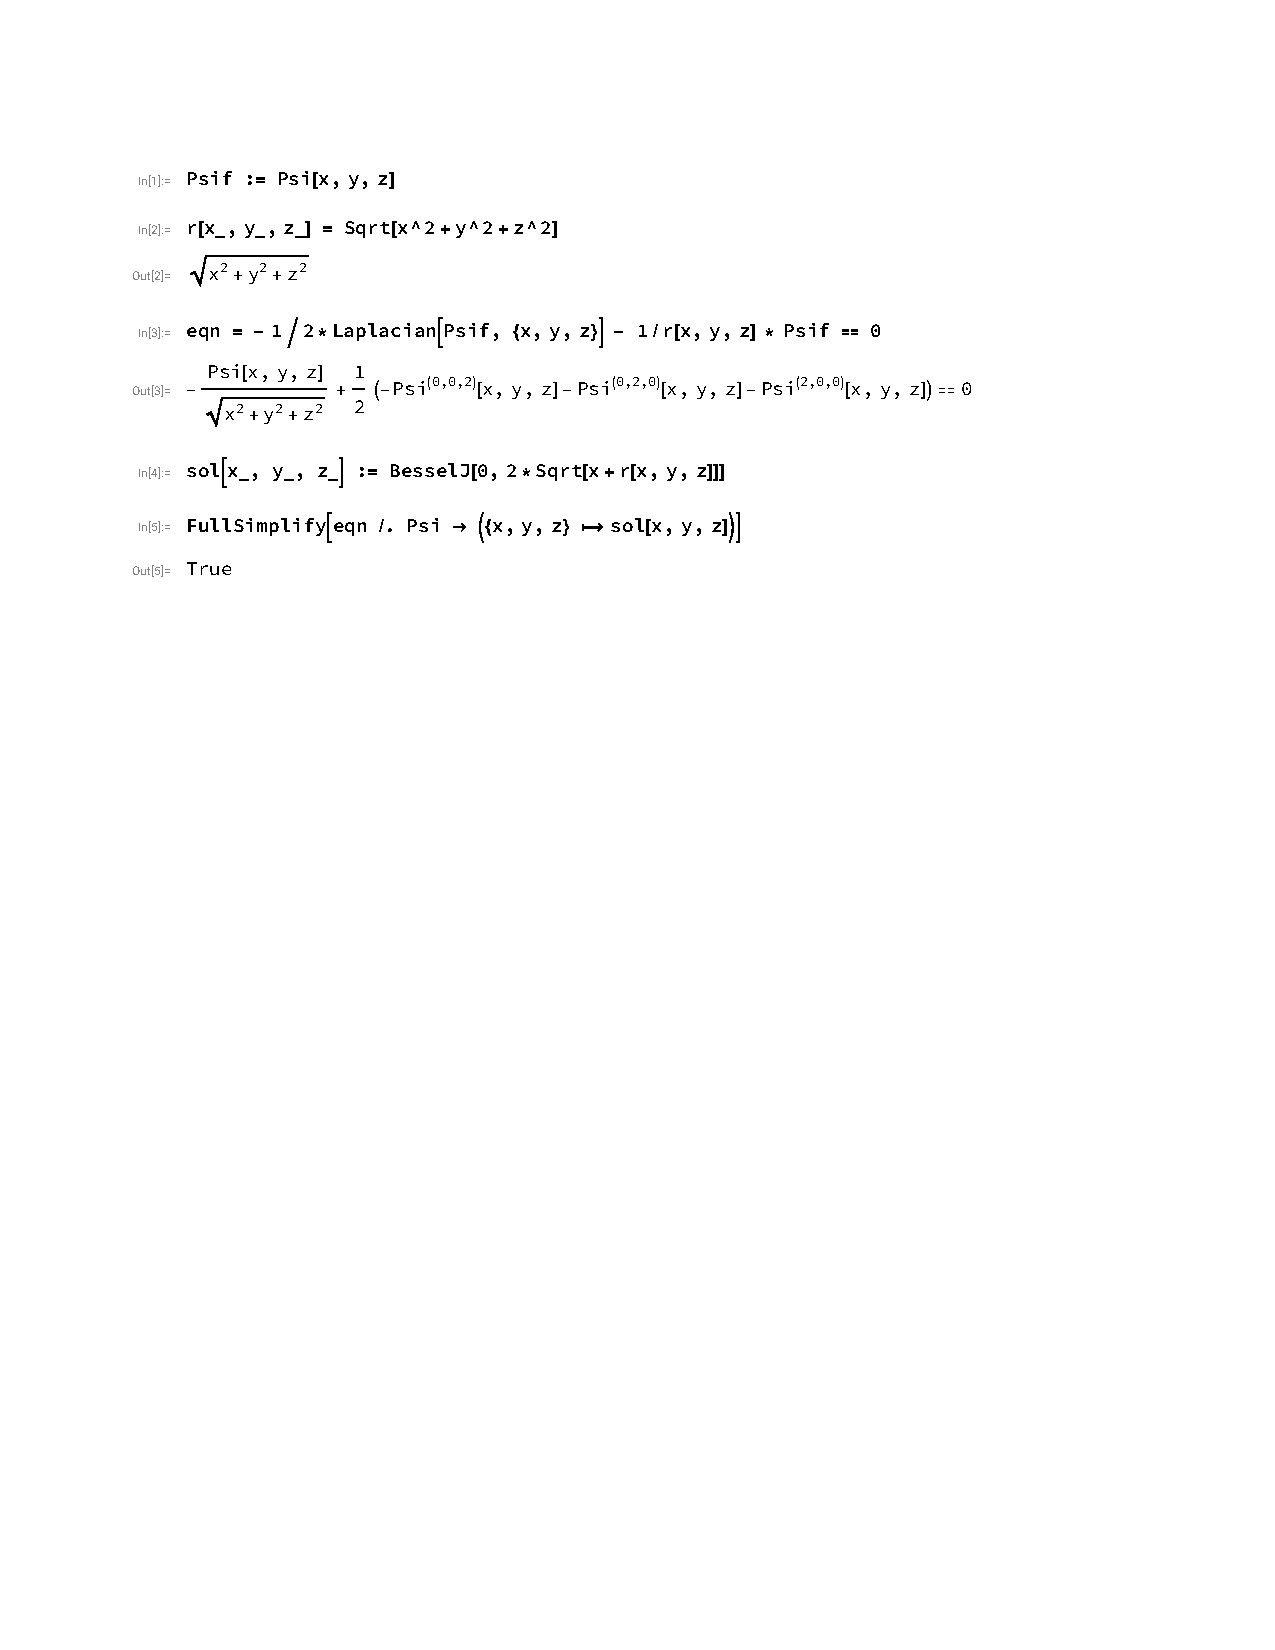
\includegraphics[page=1, clip, trim=1in 7in 1in 1in, width=\textwidth]{improved.pdf}

\subsection*{The Global Condition}

As noted in the introduction, in order to be a valid wavefunction, \eqref{L2 condition} must also be satisfied.
The physical intuition lying behind this requirement is that the square of the modulus $|\Psi|^2$ is a probability
density function and its global integral must therefore be finite, as the total probability of the electron
being somewhere is finite.

\eqref{solution} does not satisfy \eqref{L2 condition}.  This can be easily seen by inspecting \eqref{J0 definition}.
$J_0(z)$ is continuous everywhere on the real line and $J_0(0)=1$.  Also, $2\sqrt{x+r}$ is continuous
everywhere in $\mathbb{R}^3$ and is zero along the negative $x$-axis.  These facts imply that for any
$\delta>0$ there exists an $\epsilon>0$ such that $J_0(2\sqrt{x+r}) > 1-\epsilon$ for any point within
a distance of $\delta$ from the negative $x$-axis. (uniform continuity?)

This implies that for a small sphere $S$ of radius $\delta$, centered on a point along the negative $x$-axis,

\[ \int_S \left|J_0(2\sqrt{x+r})\right|^2\  dV > \frac{4}{3}\pi\delta^3(1-\epsilon) \]

Since there are an infinite number of these small spheres (disjoint?),

\[ \int_{\mathbb{R}^3} \left|J_0(2\sqrt{x+r})\right|^2\ dV  = \infty \]

and $J_0(2\sqrt{x+r})$ is not square integrable\footnote{Peter Ulrickson (Catholic University) pointed out
to me that this argument also implies that $\Psi$ is not in any $L^p$ space except $L^\infty$.}.

\subsection*{Generalization}
\parskip 12pt

Any unit vector can be picked for $(v_1, v_2, v_3)$,
so the distance in any direction from the origin can be used in lieu of $x$,
and any ordinary Bessel function can be used:

\begin{equation}
\label{generalized solution}
\Psi = F(2\sqrt{v_1 x+ v_2 y+ v_3 z+r})
\end{equation}

where

\begin{equation*}
v_1^2+v_2^2+v_3^2=1
\end{equation*}

and $F$ is any linear combination of the Bessel functions $J_0$ and $Y_0$.

By linearity of \eqref{schrodinger hydrogen}, any finite linear combination of functions of the form
\eqref{generalized solution} also solves \eqref{schrodinger hydrogen}.

The assumption that the $v_i$ coefficients are real was arbitrary.

\subsection*{Software}

The program used to construct the system of equations is available here:

\centerline{\url{https://github.com/BrentBaccala/helium}}

It's a Sage script that works fine with Sage 9.0 on Ubuntu 20.

%Use it to find the witness point \eqref{witness point} by
%running Sage as follows:
Use it to find ideal \eqref{ideal} by
running Sage as follows:

\begin{verbatim}
load('helium.sage')     # loads the script
prep_hydrogen(5)        # select PDE:hydrogen and ansatz:5
init()                  # finish setting everything up
I=ideal(eqns_RQQ)       # constuct ideal from equations
I.minimal_associated_primes()
\end{verbatim}

Here are some other convenient variables and functions in the script:

\begin{verbatim}
A, B, C, V              # trial forms of various polynomials
eq_a                    # the PDE in its original form
eq_a_convertField       # the PDE modulo the ansatz
eq_a_reduceRing_n       # the expanded numerator
R                       # polynomial ring over integers
F                       # fraction field of R
eqns_RQQ                # system of equations to solve
\end{verbatim}

%%\section*{Current Implementation Status}
\subsection*{Current Implementation Status}

The algorithm presented above can be used to check any PDE to see if any of its solutions
can be expressed using an ODE structured according to a specific ansatz.  This technique
is complementary to separation of variables, where we check a PDE to see if any of
its solutions can be expressed as a product of factors, each depending on only
a subset of the independent variables.

As my primary interest lies in quantum mechanics, I have investigated the PDEs
that model hydrogen and helium.

For hydrogen, the PDE is $\nabla^2 \Psi - \frac{1}{r} \Psi = E \Psi$

For helium, the PDE is $\nabla_1^2 \Psi + \nabla_2^2 \Psi - \frac{2}{r_1} - \Psi \frac{2}{r_2} - \Psi \frac{1}{r_{12}} \Psi = E \Psi$,
where $\Psi=\Psi(r_1,r_2,r_{12})$ and $\nabla_i$ is the Laplacian with respect to the $i^{\rm th}$ electron.
$\Psi$ is assumed to have no angular dependence, which has been known since
at least the time of Hylleraas to be a valid assumption for the ground state.

In both cases, I use Hartree atomic units to render the equations dimensionless.

\begin{comment}
Once the PDEs have been reduced modulo the differential ideal corresponding to a selected ansatz,
the resulting system of polynomial equations must be solved.  The major techniques available are:

\begin{enumerate}
\item Exact primary decomposition

This requires the computation of Gr\"obner bases, which often fails due to memory exhaustion
(oom - out of memory) and the limitations of current

\item Numerical approximation (gradient descent / Levenberg-Marquardt)

This requires extraneous ideals/varieties to be removed as they are identified.
I'm currently exploring this approach, as it is the fastest of the three,
using the DHOST algorithm to compute Euclidean Distance polynomials for
identified varieties and use this information to drive the solutions
away from identified varieties in an attempt to find new ones.

Note that this approach, while faster than the others, will never guarantee that all solutions
to the polynomial system have been found.

\item Homotopy continuation

Bertini is a major software program, but Macaulay 2 also supports homotopy continuation.
This technique is slow but, in principle, will identify all irreducible varieties.
In practice, Bertini did not identify all five irreducible varieties for hydrogen Ansatz 5.
\end{enumerate}

\end{comment}

\subsection*{Conclusion}

As we've seen, using a parameterized function space allows the use of algebraic geometry
techniques to check a PDE to see if a solution exists in that function space.
Doing so requires putting degree bounds on the various polynomials that form
the ansatz, in contrast to separation of variables, which puts no degree bounds
on the polynomials but requires the solution to be separable.  As we've seen,
even a fairly simple ansatz not only recovered a known separable solution,
but also found a previously unknown solution that is not separable.

Currently, the primary barrier to successful execution of the algorithm is
design limitations in the various software packages used to execute it.
For example, no current Gr\"obner basis algorithms, to my knowledge,
will fall back on using disk-based storage once RAM becomes exhausted.
Run times of weeks or months can be expected when searching for
truly unknown solutions to realistic problems, but no such
calculation is possible if the machine ``runs out of memory'',
even though an ample disk-based backing store may be available.

Any PDE can be explored using this technique.  For studying a
non-linear PDE such as Navier-Stokes, a different set of
ansatzen formed from non-linear ODEs might be advisable.

No theoretical treatment is currently available to predict
when these ansatzen might yield solutions.  The discovery
of a new result using such a simple ansatz suggests, however,
that even very modest degree bounds can yield solutions.

The main thrust of the author's research, however, remains
quantum mechanics and the hope of an ODE-based solution
to helium.  As of May 2023, the author continues to develop
the software tools necessary to check helium ansatz 16.6,
in the hopes of finding a solution to helium's ground state.

\subsection*{Draft Status}

This paper is still a draft and is being updated regularly.

\subsection*{Contact}

The author maintains a discussion page for this result on his personal blog at:

\begin{center}
\small
\url{https://www.freesoft.org/blogs/soapbox/a-new-solution-of-hydrogen/}
\end{center}

\begin{thebibliography}{9}
\bibitem{Bertini}
Numerically solving polynomial systems with Bertini
by D.J. Bates, J.D. Hauenstein, A.J. Sommese, and C.W. Wampler
Software, Environments, and Tools 25
SIAM, 2013

\bibitem {EHV} Eisenbud, Huneke, Vasconcelos
Direct methods for primary decomposition
David Eisenbud, Craig Huneke, and Wolmer Vasconcelos
Invent. math. 110, 207 235 (1992),
9 Springer-Verlag 1992

\bibitem{GTZ} Gianni, Trager, Zacharias
J. Symbolic Computation (1988) 6, 149-167
Gr6bner Bases and Primary Decomposition of
Polynomial Ideals
PATRIZIA GIANNI, BARRY TRAGER AND GAIL ZACHARIAS

\bibitem{Mathematica}
Wolfram Research, Inc., Mathematica, Version 14.1, Champaign, IL (2024).

\bibitem{Ritt}
J.F. Ritt, Differential Algebra, American Mathematical Society 1950

\bibitem {Schönemann}
Advanced Studies in Pure Mathematics 68, 2016
School on Real and Complex Singularities in São Carlos, 2012
pp. 171–190
Algorithms for primary decomposition in Singular
Hans Schönemann

\bibitem{SY} Localization and Primary Decomposition of Polynomial Ideals, {\it J. Symbolic Computation} (1996) {\bf 22}, 247–277

\bibitem {Wang}
{\it An Implementation of the Characteristic Set Method in Maple}
Dongming Wang,
Research Institute for Symbolic Computation,
Johannes Kepler University, A-4040 Linz, Austria

\bibitem{Watson}
{\it A Treatise On The Theory Of Bessel Functions}
Watson.

\bibitem{Wu}
Wen-Tsun, W. Basic principles of mechanical theorem proving in elementary geometries. J Autom Reasoning 2, 221–252 (1986). https://doi.org/10.1007/BF02328447

\end{thebibliography}

\vfill\eject
\subsection*{Appendix: Manual Verification of the Result}
For anybody wondering how Mathematica concludes that \eqref{solution} solves \eqref{schrodinger hydrogen},
the claim is that $\Psi = J_0(2\sqrt{x+r}) = (J_0 \circ 2\sqrt{v}) (x+r)$ satisfies:

\begin{equation}
\label{claim}
\left(\frac{\delta^2}{\delta^2 x} + \frac{\delta^2}{\delta^2 y} + \frac{\delta^2}{\delta^2 z}\right) \Psi + \frac{2}{r}\Psi = 0
\end{equation}

\vskip 12pt

Letting $v=x+r$, we compute the first partial derivatives of $\Psi$:

\begin{equation}
\begin{gathered}
\frac{\delta \Psi}{\delta x} = \frac{d v}{d x} \frac{d}{d v} \left(J_0 \circ 2\sqrt{v}\right) = \frac{d v}{d x} J_0'(2\sqrt{v}) v^{-1/2} \\
\frac{\delta \Psi}{\delta y} = \frac{d v}{d y} \frac{d}{d v} \left(J_0 \circ 2\sqrt{v}\right) = \frac{d v}{d y} J_0'(2\sqrt{v}) v^{-1/2} \\
\frac{\delta \Psi}{\delta z} = \frac{d v}{d z} \frac{d}{d v} \left(J_0 \circ 2\sqrt{v}\right) = \frac{d v}{d z} J_0'(2\sqrt{v}) v^{-1/2}
\end{gathered}
\end{equation}

\vskip 12pt

Next we compute the partial second derivatives of $\Psi$:

\begin{equation}
\label{second partials}
\begin{gathered}
\frac{\delta^2 \Psi}{\delta x^2} = \frac{d^2 v}{d x^2} J_0'(2\sqrt{v}) v^{-1/2} + \left(\frac{d v}{d x}\right)^2 J_0''(2\sqrt{v}) v^{-1} - \frac{1}{2} \left(\frac{d v}{d x}\right)^2 J_0'(2\sqrt{v}) v^{-3/2} \\
\frac{\delta^2 \Psi}{\delta y^2} = \frac{d^2 v}{d y^2} J_0'(2\sqrt{v}) v^{-1/2} + \left(\frac{d v}{d y}\right)^2 J_0''(2\sqrt{v}) v^{-1} - \frac{1}{2} \left(\frac{d v}{d y}\right)^2 J_0'(2\sqrt{v}) v^{-3/2} \\
\frac{\delta^2 \Psi}{\delta z^2} = \frac{d^2 v}{d z^2} J_0'(2\sqrt{v}) v^{-1/2} + \left(\frac{d v}{d z}\right)^2 J_0''(2\sqrt{v}) v^{-1} - \frac{1}{2} \left(\frac{d v}{d z}\right)^2 J_0'(2\sqrt{v}) v^{-3/2}
\end{gathered}
\end{equation}

\vskip 12pt

We need to know the derivatives of $v=r+x$ with respect to the coordinates:

\vskip 12pt

\begin{equation}
\label{first v}
\begin{gathered}
\frac{d v}{d x} = \frac{d}{d x} (x+r) = 1 + \frac{x}{r} \\
\frac{d v}{d y} = \frac{d}{d y} (x+r) = \frac{y}{r} \\
\frac{d v}{d z} = \frac{d}{d z} (x+r) = \frac{z}{r}
\end{gathered}
\end{equation}

\vskip 12pt

\begin{equation}
\label{second v}
\begin{gathered}
\frac{d^2 v}{d x^2} = \frac{d}{d x} \left(1 + \frac{x}{r}\right) = \frac{r - x(x/r)}{r^2} = \frac{r^2 - x^2}{r^3} \\
\frac{d^2 v}{d y^2} = \frac{r^2 - y^2}{r^3} \\
\frac{d^2 v}{d z^2} = \frac{r^2 - z^2}{r^3}
\end{gathered}
\end{equation}

\vskip 20pt

Substituting \eqref{first v} and \eqref{second v} into \eqref{second partials}, and \eqref{second partials}
into the LHS of \eqref{claim}, we obtain:

\begin{equation*}
\begin{aligned}
&\frac{d^2 v}{d x^2} J_0'(2\sqrt{v}) v^{-1/2} + \left(\frac{d v}{d x}\right)^2 J_0''(2\sqrt{v}) v^{-1} - \frac{1}{2} \left(\frac{d v}{d x}\right)^2 J_0'(2\sqrt{v}) v^{-3/2} \\
+& \frac{d^2 v}{d y^2} J_0'(2\sqrt{v}) v^{-1/2} + \left(\frac{d v}{d y}\right)^2 J_0''(2\sqrt{v}) v^{-1} - \frac{1}{2} \left(\frac{d v}{d y}\right)^2 J_0'(2\sqrt{v}) v^{-3/2} \\
+& \frac{d^2 v}{d z^2} J_0'(2\sqrt{v}) v^{-1/2} + \left(\frac{d v}{d z}\right)^2 J_0''(2\sqrt{v}) v^{-1} - \frac{1}{2} \left(\frac{d v}{d z}\right)^2 J_0'(2\sqrt{v}) v^{-3/2} \\
+& \frac{2}{r} J_0(2\sqrt{v})
\end{aligned}
\end{equation*}

\begin{equation*}
\begin{aligned}
=&\frac{r^2-x^2}{r^3} J_0'(2\sqrt{v}) v^{-1/2} + (1+\frac{x}{r})^2 J_0''(2\sqrt{v}) v^{-1} - \frac{1}{2} (1+\frac{x}{r})^2 J_0'(2\sqrt{v}) v^{-3/2} \\
&+ \frac{r^2-y^2}{r^3} J_0'(2\sqrt{v}) v^{-1/2} + \left(\frac{y}{r}\right)^2 J_0''(2\sqrt{v}) v^{-1} - \frac{1}{2} \left(\frac{y}{r}\right)^2 J_0'(2\sqrt{v}) v^{-3/2} \\
&+ \frac{r^2-z^2}{r^3} J_0'(2\sqrt{v}) v^{-1/2} + \left(\frac{z}{r}\right)^2 J_0''(2\sqrt{v}) v^{-1} - \frac{1}{2} \left(\frac{z}{r}\right)^2 J_0'(2\sqrt{v}) v^{-3/2} \\
&+ \frac{2}{r} J_0(2\sqrt{v})
\end{aligned}
\end{equation*}

\begin{equation*}
\begin{aligned}
=&\frac{3r^2-x^2-y^2-z^2}{r^3} J_0'(2\sqrt{v}) v^{-1/2} + (1+2\frac{x}{r} +\frac{x^2}{r^2} + \frac{y^2}{r^2} + \frac{z^2}{r^2}) J_0''(2\sqrt{v}) v^{-1} \\
&- \frac{1}{2} (1+2\frac{x}{r} +\frac{x^2}{r^2}+ \frac{y^2}{r^2} + \frac{z^2}{r^2}) J_0'(2\sqrt{v}) v^{-3/2}
+ \frac{2}{r} J_0(2\sqrt{v})
\end{aligned}
\end{equation*}

\begin{equation*}
=\frac{2}{r} J_0'(2\sqrt{v}) v^{-1/2} + (2+2\frac{x}{r}) J_0''(2\sqrt{v}) v^{-1} - \frac{1}{2} (2+2\frac{x}{r}) J_0'(2\sqrt{v}) v^{-3/2} + \frac{2}{r} J_0(2\sqrt{v})
\end{equation*}

\begin{equation*}
=\frac{2}{r} J_0'(2\sqrt{v}) v^{-1/2} + 2\frac{x+r}{r} J_0''(2\sqrt{v}) v^{-1} - \frac{x+r}{r} J_0'(2\sqrt{v}) v^{-3/2}
+ \frac{2}{r} J_0(2\sqrt{v})
\end{equation*}

Remembering that $v=x+r$,

%%\begin{equation*}
%%=\frac{2}{r} J_0'(2\sqrt{v}) v^{-1/2} + 2\frac{x+r}{r} J_0''(2\sqrt{v}) v^{-1} - \frac{1}{r} J_0'(2\sqrt{v}) v^{-1/2}
%%+ \frac{2}{r} J_0(2\sqrt{v})
%%\end{equation*}

\begin{equation*}
=\frac{2}{r} J_0'(2\sqrt{v}) v^{-1/2} + \frac{2}{r} J_0''(2\sqrt{v}) - \frac{1}{r} J_0'(2\sqrt{v}) v^{-1/2}
+ \frac{2}{r} J_0(2\sqrt{v})
\end{equation*}

\begin{equation*}
=\frac{2}{r} J_0''(2\sqrt{v}) + \frac{1}{r} J_0'(2\sqrt{v}) v^{-1/2} + \frac{2}{r} J_0(2\sqrt{v})
\end{equation*}

\begin{equation*}
=\frac{2}{r} J_0''(2\sqrt{v}) + \frac{2}{r\cdot2\sqrt{v}} J_0'(2\sqrt{v}) + \frac{2}{r} J_0(2\sqrt{v})
\end{equation*}

\begin{equation}
\label{last eq in derivation}
=\frac{2}{r} \left( J_0''(2\sqrt{v}) + \frac{1}{2\sqrt{v}} J_0'(2\sqrt{v}) + J_0(2\sqrt{v})\right)
\end{equation}

Now, the ordinary Bessel function $J_0(x)$ satisfies:

\begin{equation*}
x^2 J_0''(x) + xJ_0'(x) + x^2J_0(x) = 0
\end{equation*}

dividing through by $x^2$ and changing variables, we get:

\begin{equation*}
J_0''(2\sqrt{v}) + \frac{1}{2\sqrt{v}}J_0'(2\sqrt{v}) + J_0(2\sqrt{v}) = 0
\end{equation*}

which shows that \eqref{last eq in derivation} is zero, and establishes the proof of \eqref{claim}.

\end{document}
